\section{Typed Guided Adversarial Testing}

\begin{figure}[th!]
    \centering
    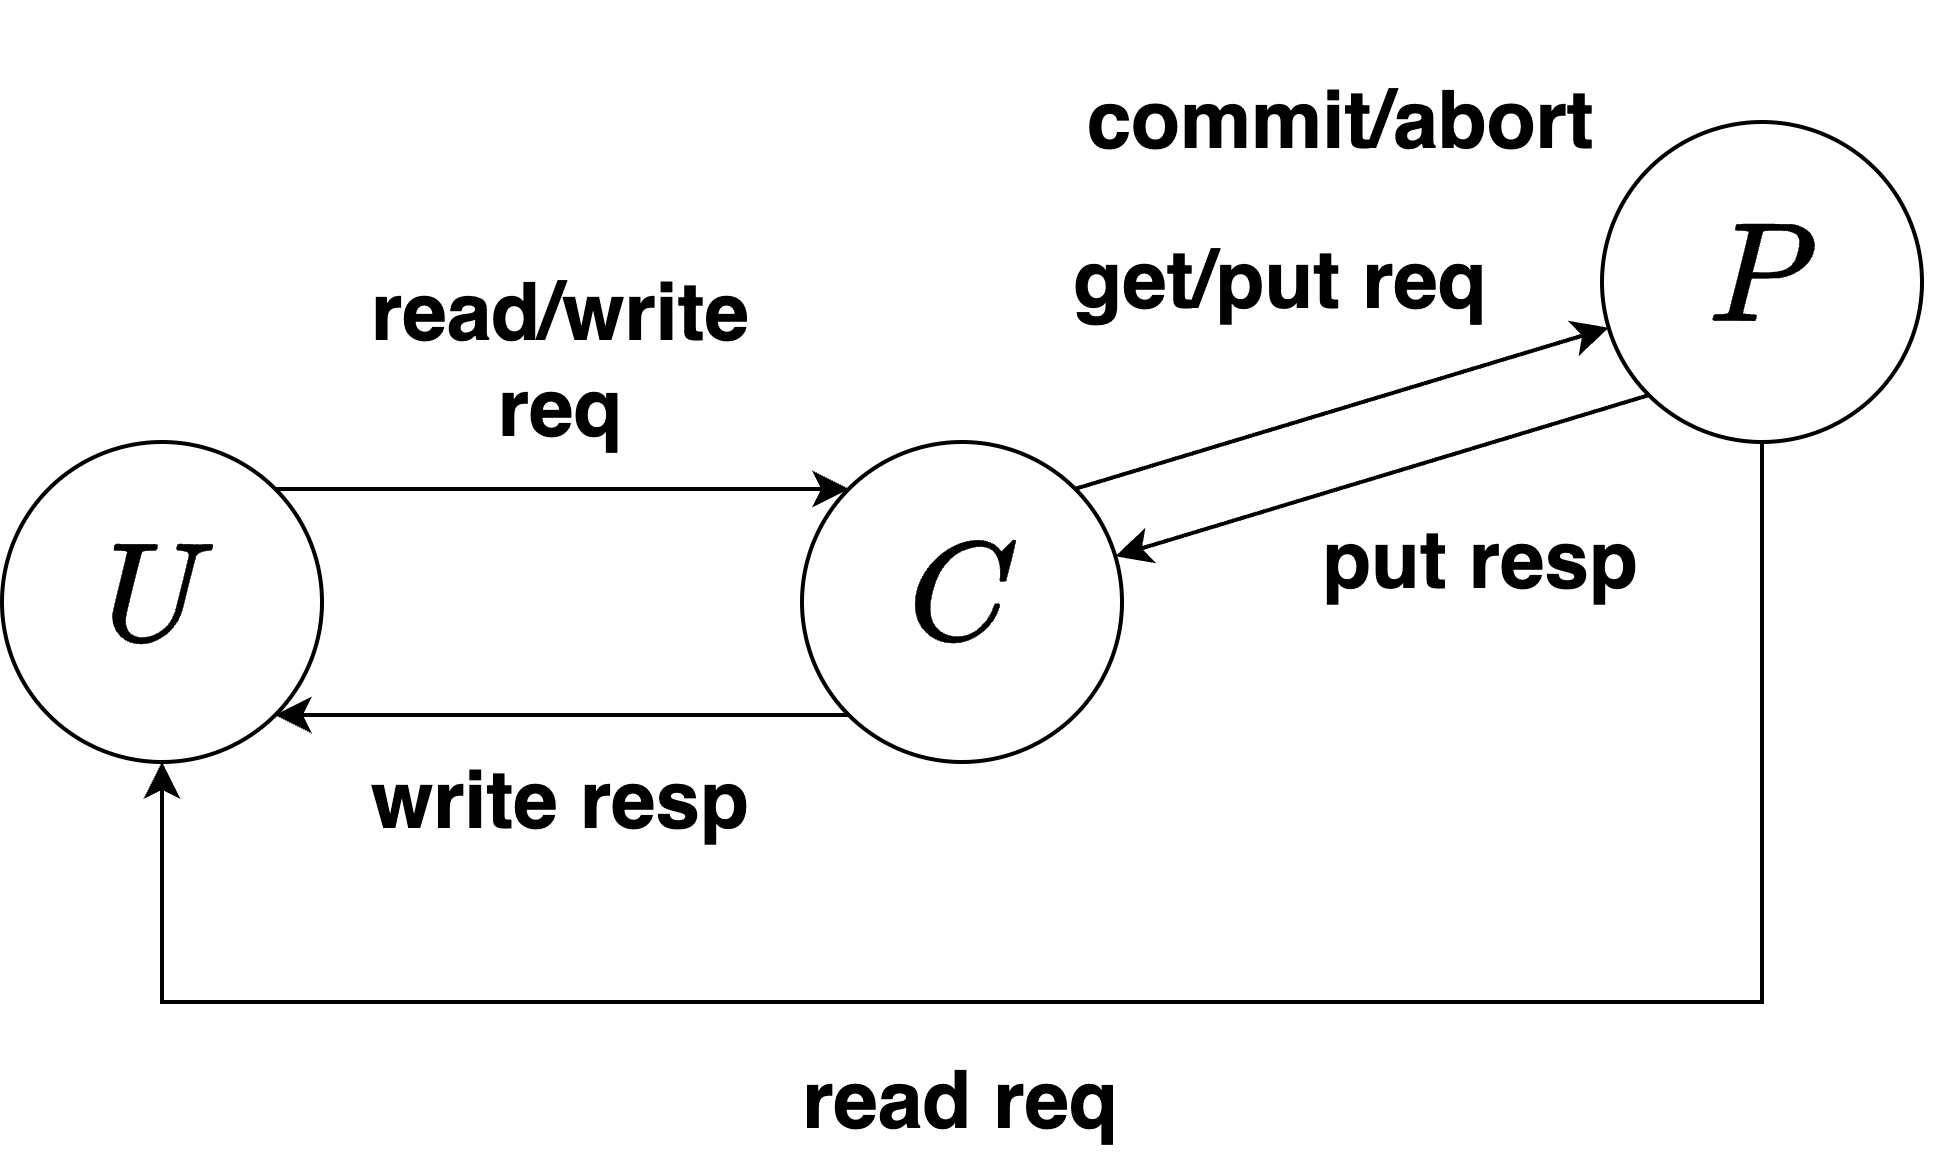
\includegraphics[width=0.4\linewidth]{figures/typed-guided-test.drawio.png}
    \caption{Caption}
    \label{fig:enter-label}
\end{figure}

\paragraph{Message} The messages definition is shown below. Each message should contains two fields $\Code{\#src}$ and  $\Code{\#dst}$ to indicate the source machine and destination machine, which are omitted.

\begin{minted}[xleftmargin=5pt, numbersep=4pt, linenos = true, fontsize = \footnotesize, escapeinside=??]{OCaml}
type payload =
(* user <--> coordinator *)
  | WriteReq of { v : int }
  | WriteResp of { v : int; stat : bool }
  | ReadReq
(* user <--> participant *)
  | ReadResp of { v : int }
(* coordinator <--> participant *)
  | GetReq
  | PutReq of { v : int }
  | PutResp of { stat : bool }
  | Abort
  | Commit
(* dummy message *)
  | Gen
\end{minted}

\begin{figure}[t!]
{\footnotesize
{\small\begin{flalign*}
 &\text{\textbf{Specification Syntax}} &
\end{flalign*}}
\vspace{-1.8em}
{\small
\begin{alignat*}{2}
    \text{\textbf{Message }}& \quad & \textbf{msg} ::= \quad & \msg{op}{\phi}
    \\\text{\textbf{SFA }}& \quad & A ::= \quad & \emptyset ~|~ \epsilon ~|~ \textbf{msg} ~|~ A \lor A ~|~ A;A ~|~ A*
    % \\\text{\textbf{Event }}& \quad & \textbf{ev} ::= \quad & \Code{send}\; \textbf{msg} ~|~ \Code{receive}\; \textbf{msg}
    \\\text{\textbf{HAT }}& \quad & \tau ::= \quad & \hpair{A}{A} ~|~ x{:}t \sarr \tau ~|~ x{:}t \garr \tau ~|~ \tau \interty \tau
  \end{alignat*}}
\caption{\langname{} types.}}
\label{fig:type-syntax}
\vspace{-.2cm}
\end{figure}

\paragraph{Types} The types of these interfaces are shown below, the syntax is defined in \autoref{fig:type-syntax}.



{\footnotesize\begin{align*}
    &\Code{ReadReq}: \hpair{\msg{GetReq}{\Code{\top }}}{\anyA^*}
    \\&\Code{GetReq}:  \forall v{:}\nuot{int}{\vnu \not= 0}.\hpair{\msg{ReadRsp}{ \Code{\#v = }v }}{\finalA \msg{putReq}{\Code{\#v = }v}}
    \\&\Code{GetReq}:  \hpair{\msg{ReadRsp}{ \Code{\#v = 0}}}{\finalA \msg{putReq}{\Code{\#v = 0}} \lor \neg\finalA \msg{putReq}{\top}}
    \\
    \\&\Code{WriteReq}:  \Code{v{:}int} \sarr \hpair{\msg{PutReq}{\Code{\#v = v} }^+}{\anyA^*}
    \\&\Code{PutReq}:  \Code{v{:}int} \sarr \hpair{\msg{PutRsp}{\top}}{\anyA^*}
    \\&\Code{PutRsp}:  \Code{v{:}int} \sarr \Code{stat{:}bool} \sarr \hpair{\epsilon}{\anyA^*}
    \\&\Code{PutRsp}:  \Code{v{:}int} \sarr \Code{stat{:}}\nuot{bool}{\neg\vnu} \sarr \hpair{
    \msg{Abort}{\top}^+;
    \msg{WriteRsp}{\Code{\#v = v}\land \neg\Code{\#stat}}}{\anyA^*}
    \\&\Code{PutRsp}:  \Code{v{:}int} \sarr \Code{stat{:}}\nuot{bool}{\vnu} \sarr 
    \\&\;\; \hpair{
    \msg{Commit}{\top}^+;
    \msg{WriteRsp}{\Code{\#v = v} \land \Code{\#stat}}}{\neg\finalA\msg{PutRsp}{ \neg \Code{\#stat}}}
    \\&\Code{PutRsp}:  \Code{v{:}int} \sarr \Code{stat{:}bool} \sarr 
    \\&\;\; \hpair{
    \msg{Abort}{\top}^+;
    \msg{WriteRsp}{\Code{\#v = v} \land \neg\Code{\#stat}}}{\finalA\msg{PutRsp}{ \neg \Code{\#stat}}}
\end{align*}}

The denotation $\Code{msg} {:} \hpair{B}{A}$ is in over- and reverse style.
\begin{align*}
    \forall \alpha\;\beta. \beta \in B \land \alpha \models \Code{msg} \xrightarrow{send} \beta \impl \alpha \in A
\end{align*}\noindent
It means that ``if we prune out precondition $\neg A$, we don't lose compeletness''.

\paragraph{Correctness Property} The correctness property is shown below.
{\footnotesize\begin{align*}
    \forall \Code{v{:}int}.\neg (\anyA^*;&\Code{receive}\;\msg{ReadRsp}{\Code{ \#v = v}};(\anyA \setminus \Code{receive}\;\msg{WriteRsp}{\Code{ \#stat}})^*; 
    \\&\Code{receive}\;\msg{ReadRsp}{\Code{ \#v \not= v}};(\anyA \setminus \Code{receive}\;\msg{WriteRsp}{\Code{ \#stat}})^*)
\end{align*}}\noindent
The incorrectness property is
{\footnotesize\begin{align*}
    \exists \Code{v{:}int}.\anyA^*;&\Code{receive}\;\msg{ReadRsp}{\Code{ \#v = v}};(\anyA \setminus \Code{receive}\;\msg{WriteRsp}{\Code{ \#stat}})^*; 
    \\&\Code{receive}\;\msg{ReadRsp}{\Code{ \#v \not= v}};(\anyA \setminus \Code{receive}\;\msg{WriteRsp}{\Code{ \#stat}})^*
\end{align*}}\noindent


\paragraph{Counterexample} The correctness property is shown below. When the \Code{Coordinator} decides to commit a value, two read requests may read the previous and updated value in a specific message interleaving.
\begin{minted}[xleftmargin=5pt, numbersep=4pt, linenos = true, fontsize = \footnotesize, escapeinside=??]{OCaml}
[User] --(WriteReq {v = 2})--> [Coordinator]
[Coordinator] --(PutReq {v = 2})--> [Participant0]
[User] --(ReadReq {clientId = 3})--> [Coordinator]
[Coordinator] --(PutReq {v = 2})--> [Participant1]
[Participant0] --(PutResp {stat = true})--> [Coordinator]
[Participant1] --(PutResp {stat = true})--> [Coordinator]
[Coordinator] --(Commit)--> [Participant1]
[Coordinator] --(WriteResp {v = 2; stat = true})--> [User] (* Client finds writte success *)
[User] --(ReadReq {clientId = 3})--> [Coordinator]
[Coordinator] --(GetReq {clientId = 3})--> [Participant0] (* get P0 *)
[Coordinator] --(Commit)--> [Participant0] (* commit P0 *)
[Participant0] --(ReadResp {v = 0})--> [User]
[Coordinator] --(GetReq {clientId = 3})--> [Participant0] (* get P0 *)
[Participant1] --(ReadResp {v = 2})--> [User]
\end{minted}

\begin{figure}[t!]
{\footnotesize
{\small\begin{flalign*}
 &\text{\textbf{Specification Syntax}} &
\end{flalign*}}
\vspace{-1.8em}
{\small
\begin{alignat*}{2}
    \\\text{\textbf{SFA }}& \quad & A ::= \quad & \emptyset ~|~ \epsilon ~|~ \textbf{msg} ~|~ A \lor A ~|~ A;A ~|~ A*
    \\\text{\textbf{Incor SFA}}& \quad & \mathcal{A} ::= \quad & \epsilon ~|~ \msg{op}{\overline{x}} ~|~ \boxed{A} ~|~ \mathcal{A};\mathcal{A}
  \end{alignat*}}
\caption{\langname{} types.}}\label{fig:type-syntax2}
\vspace{-.2cm}
\end{figure}

\paragraph{Intuition} The incorrectness property is similar with the counterexample trace enough, besides three differences: 1) the existential quantified $v$ 2) the Kleene star 3) the union (i.e. $\anyA$). We try to instantiate this automata into a trace step by step. As shown in \autoref{fig:type-syntax2}, the incorrectness-style automata encapsulates the union and Kleene star into the box $\boxed{A}$. We also extract the local variables into type context to instantiate them later.
{\footnotesize\begin{align*}
    \Code{v_0}{:}\nuut{int}{\top}, \Code{v_1}{:}\nuut{int}{\vnu != \Code{v_0}} \vdash \boxed{\anyA^*};&\Code{receive}\;\msg{ReadRsp}{\Code{ \#v = v_0}};\boxed{(\anyA \setminus \Code{receive}\;\msg{WriteRsp}{\Code{ \#stat}})^*}; 
    \\&\Code{receive}\;\msg{ReadRsp}{\Code{ \#v = v_1}};\boxed{(\anyA \setminus \Code{receive}\;\msg{WriteRsp}{\Code{ \#stat}})^*}
\end{align*}}\noindent
The $\Code{receive}\;\msg{ReadRsp}{\Code{ \#v \not= v}}$ indicates a $\Code{ReadRsp}$ is sent; according to the types, handling $\Code{ReadReq}$ can generate $\Code{ReadRsp}$. The denotation $\Code{msg} {:} \hpair{B}{A}$ is in over- and reverse style.
\begin{align*}
    \forall \alpha\;\beta. \beta \in B \land \alpha \models \Code{msg} \xrightarrow{send} \beta \impl \alpha \in A
\end{align*}\noindent
It means that ``if we prune out precondition $\neg A$, we don't lose compeletness''. It is weaker than incorrectness triple. Now we have no idea which type we should use, it depends on if $\Code{v}$ is equal to $0$. Now assume $\Code{v = 0}$

\begin{prooftree}
\hypo{ }
\infer1[\textsc{TWeak}]{
\Gamma, \nuut{unit}{\phi} \vdash \mathcal{A} \typeinfer \Gamma \vdash \mathcal{A}
}
\end{prooftree}

Then we have
{\footnotesize\begin{align*}
    \Code{v_0}{:}\nuut{int}{\vnu = 0}, \Code{v_1}{:}\nuut{int}{\vnu != \Code{v_0}} \vdash \boxed{\anyA^*};&\Code{receive}\;\msg{ReadRsp}{\Code{ \#v = v_0}};\boxed{(\anyA \setminus \Code{receive}\;\msg{WriteRsp}{\Code{ \#stat}})^*}; 
    \\&\Code{receive}\;\msg{ReadRsp}{\Code{ \#v = v_1}};\boxed{(\anyA \setminus \Code{receive}\;\msg{WriteRsp}{\Code{ \#stat}})^*}
\end{align*}}\noindent
In order to receive $\Code{receive}\;\msg{ReadRsp}{\Code{ \#v = v}}$, we need receive $\Code{GetReq}$ after $\finalA \msg{putReq}{\Code{\#v = 0}} \lor \neg\finalA \msg{putReq}{\top}$. If implies that we should do a backward inference.

{\small
\begin{prooftree}
\hypo{
\parbox{20mm}{\center
$A' = A_1;B;A_2$\quad
$\Gamma \vdash A' \subseteq A$
}}
\infer1[\textsc{SpecializeMid}]{
\Gamma \vdash A' \sqsubseteq_{mid} (A, B)
}
\end{prooftree} 
\quad
\begin{prooftree}
\hypo{
\parbox{20mm}{\center
$A' = B;A_2$\quad
$\Gamma \vdash A' \subseteq A$
}}
\infer1[\textsc{SpecializePre}]{
\Gamma \vdash A' \sqsubseteq_{pre} (A, B)
}
\end{prooftree} 
\quad
\begin{prooftree}
\hypo{
\parbox{20mm}{\center
$A' = A_2;B$\quad
$\Gamma \vdash A' \subseteq A$
}}
\infer1[\textsc{SpecializePost}]{
\Gamma \vdash A' \sqsubseteq_{post} (A, B)
}
\end{prooftree} 
\\ \ \\ \ \\ \ 
\begin{prooftree}
\hypo{
\parbox{80mm}{\center
$\vdash \mathbf{msg'} : \hpair{A}{B}$\quad
$\Gamma \vdash A' \sqsubseteq_{mid} (A, \mathbf{msg})$\quad
$\Gamma \vdash \mathcal{A}_{1}' \sqsubseteq_{pre} (\mathcal{A}_1, B;\mathbf{msg'};A')$
}}
\infer1[\textsc{TApp}]{
\Gamma \vdash \mathcal{A}_{1}';\mathbf{msg};\mathcal{A}_2 \typeinfer \Gamma \vdash \mathcal{A}_1;\mathbf{msg};\mathcal{A}_2
}
\end{prooftree}
}

Then we have
{\footnotesize\begin{align*}
    \Code{v_0}{:}\nuut{int}{\vnu = 0}, \Code{v_1}{:}\nuut{int}{\vnu != \Code{v_0}} \vdash &\boxed{(\finalA \msg{putReq}{\Code{\#v = 0}} \lor \neg\finalA \msg{putReq}{\top});\Code{GetReq};\Code{send\;}\msg{ReadRsp}{\Code{ \#v = v}};\anyA^*};
    \\&\msg{ReadRsp}{\Code{ \#v = v_0}};\boxed{(\anyA \setminus \msg{WriteRsp}{\Code{ \#stat}})^*}; 
    \\&\msg{ReadRsp}{\Code{ \#v = v_1}};\boxed{(\anyA \setminus \msg{WriteRsp}{\Code{ \#stat}})^*}
\end{align*}}\noindent
We also want to eliminate union

\begin{prooftree}
\hypo{ }
\infer1[\textsc{TUnion}]{
\Gamma \vdash \mathcal{A}_1;\boxed{A_1};\mathcal{A}_2  \typeinfer \Gamma \vdash \mathcal{A}_1;\boxed{A_1 \lor A_2};\mathcal{A}_2
}
\end{prooftree}

Then we have
{\footnotesize\begin{align*}
    \Code{v_0}{:}\nuut{int}{\vnu = 0}, \Code{v_1}{:}\nuut{int}{\vnu != \Code{v_0}} \vdash &\boxed{(\anyA \setminus \msg{putReq}{\top})^*}\Code{GetReq};\Code{send\;}\msg{ReadRsp}{\Code{ \#v = v}};\boxed{\anyA^*};
    \\&\msg{ReadRsp}{\Code{ \#v = v_0}};\boxed{(\anyA \setminus \msg{WriteRsp}{\Code{ \#stat}})^*}; 
    \\&\msg{ReadRsp}{\Code{ \#v = v_1}};\boxed{(\anyA \setminus \msg{WriteRsp}{\Code{ \#stat}})^*}
\end{align*}}\noindent

We apply \textsc{TApp} to \Code{GetReq}, it can be sent by \Code{ReadReq}, then we have

{\footnotesize\begin{align*}
    \Code{v_0}{:}\nuut{int}{\vnu = 0}, \Code{v_1}{:}\nuut{int}{\vnu != \Code{v_0}} \vdash &\boxed{(\anyA \setminus \msg{putReq}{\top})^*};\Code{ReadReq};\Code{send\;}\Code{GetReq};\boxed{(\anyA \setminus \msg{putReq}{\top})^*};
    \\&\Code{GetReq};\Code{send\;}\msg{ReadRsp}{\Code{ \#v = v}};\boxed{\anyA^*};
    \\&\msg{ReadRsp}{\Code{ \#v = v_0}};\boxed{(\anyA \setminus \msg{WriteRsp}{\Code{ \#stat}})^*}; 
    \\&\msg{ReadRsp}{\Code{ \#v = v_1}};\boxed{(\anyA \setminus \msg{WriteRsp}{\Code{ \#stat}})^*}
\end{align*}}\noindent

We do similar things to the second read response, which need the following prefix:
{\footnotesize\begin{align*}
    ...;\msg{WriteReq}{\Code{\#v = v_1}};...;\msg{putReq}{\Code{\#v = v_1}}; ...;\Code{GetReq};\Code{send\;}\msg{ReadRsp}{\Code{ \#v = v_1}}; ... ;\msg{ReadRsp}{\Code{ \#v = v_1}};
\end{align*}}\noindent
Note that, we use the first specification of \Code{GetReq} which has an universal quantified $\forall v$, that is instantiated into $v_1$. We don't know which box should we instantiates this trace, actually, we find that the first and second box doesn't contain $\Code{putReq}$, thus we choose to use the third one. There should be a rule to do it...

% \Code{GetReq};\Code{send\;}\msg{ReadRsp}{\Code{ \#v = v}};

{\footnotesize\begin{align*}
    \Code{v_0}{:}\nuut{int}{\vnu = 0}, \Code{v_1}{:}\nuut{int}{\vnu != \Code{v_0}} \vdash &\boxed{(\anyA \setminus \msg{putReq}{\top})^*};\Code{ReadReq};\Code{send\;}\Code{GetReq};\boxed{(\anyA \setminus \msg{putReq}{\top})^*};
    \\&\Code{GetReq};\Code{send\;}\msg{ReadRsp}{\Code{ \#v = v}};\boxed{\anyA^*};
    \\&\msg{WriteReq}{\Code{\#v = v_1}};\boxed{\anyA^*};\textcolor{red}{\boxed{\msg{putReq}{\Code{\#v = v_1}}^+}};\boxed{\anyA^*};
    \\&\Code{ReadReq};\Code{GetReq};\Code{send\;}\msg{ReadRsp}{\Code{ \#v = v_1}}; \boxed{\anyA^*} ;
    \\&\msg{ReadRsp}{\Code{ \#v = v_0}};\boxed{(\anyA \setminus \msg{WriteRsp}{\Code{ \#stat}})^*}; 
    \\&\msg{ReadRsp}{\Code{ \#v = v_1}};\boxed{(\anyA \setminus \msg{WriteRsp}{\Code{ \#stat}})^*}
\end{align*}}\noindent
Note that we have no idea how many \Code{putReq} are sent, which is controlled by the implementation. Thus, we should run test until we see how many messages are sent. Moreover, we can dynamically instantiate the quantified variables.

\begin{prooftree}
\hypo{ \vdash \alpha \in \mathcal{A} \quad \alpha \text{ is a realizable trace} }
\infer1[\textsc{TTest}]{
\vdash \alpha;\mathcal{A}' \typeinfer \Gamma \vdash \mathcal{A};\mathcal{A}'
}
\end{prooftree}

The followings trace is valid:
\begin{align*}
    \Code{ReadReq};\Code{GetReq};\msg{WriteReq}{\Code{\#v = 2}};(\Code{send}\; \msg{putReq}{\Code{\#v = v_1}});(\Code{send}\; \msg{putReq}{\Code{\#v = v_1}})
\end{align*}

We continue the type check:
{\footnotesize\begin{align*}
    \vdash &\Code{ReadReq};\Code{GetReq};\msg{WriteReq}{\Code{\#v = 2}};(\Code{send}\; \msg{putReq}{\Code{\#v = v_1}});(\Code{send}\; \msg{putReq}{\Code{\#v = v_1}})
    \\&;\boxed{\anyA^*};\msg{putReq}{\Code{\#v = 2}};\boxed{\anyA^*};\msg{putReq}{\Code{\#v = 2}};\boxed{\anyA^*};
    \\&\Code{ReadReq};\Code{GetReq};\Code{send\;}\msg{ReadRsp}{\Code{ \#v = 2}}; \boxed{\anyA^*} ;
    \\&\msg{ReadRsp}{\Code{ \#v = 0}};\boxed{(\anyA \setminus \msg{WriteRsp}{\Code{ \#stat}})^*}; 
    \\&\msg{ReadRsp}{\Code{ \#v = 2}};\boxed{(\anyA \setminus \msg{WriteRsp}{\Code{ \#stat}})^*}
\end{align*}}\noindent
We also know $\Code{WriteResp}$ cannot be received at the end of trace, thus the scheduler should schedule it easiler.